\begin{tikzpicture}
    \begin{axis}[
        width  = \textwidth,
        height = 0.3\textheight,
        major x tick style = transparent,
        ybar,
        bar width=10pt,
        ymajorgrids = true,
        ylabel = {Feature importance},
        xtick = {1,2,3,4,5,6},
        xticklabel style={align=center},
        xticklabels = {Surface\\solar\\rad down, Surface\\thermal\\rad down, Top net\\solar rad, Total\\precipitation, Total\\cloud cover, Previous\\points},
        scaled y ticks = false,
    ]
        \addplot
            coordinates {(1, 1.3365) (2, 1.0214) (3, 1.0199) (4, 1.0020) (5, 1.0025)};
        \addplot
            coordinates {(1, 1.2202) (2, 1.0052) (3, 1.0856) (4, 1.0032) (5, 1.0405)};
        \addplot
            coordinates {(1, 1.0268) (2, 1.0208) (3, 1.0516) (4, 1.0124) (5, 1.2059) (6, 1.0918)};

        \legend{QRF, NNQF, SQF-RNN}
    \end{axis}
\end{tikzpicture}